\section{Reaction mechanism of the fabrication methods for PLA}

A very common used bio-based polymer is \gls{pla}. The two best know pathways to synthesize \gls{pla} are via a \gls{rop} or polycondensation. 
These two different routes to form \gls{pla} start from the monomer \gls{la} for which two optically active stereoisomers exists, namely the naturally occuring L-\gls{la} (S configuration) and the manufactured D-\gls{la} (R-configuration)(fig. \ref{fig:LA_types}). 
Pure L- and D-\gls{la} are generally synthesized by fermentation using suitable micro-organisms but the recamic DL-\gls{la} (RS configuration) is conventiently synthesize by a chemical method and shows some characteristic differences from the optically active ones\citec{MASUTANI201411}.

\begin{figure}[ht]
    \centering
    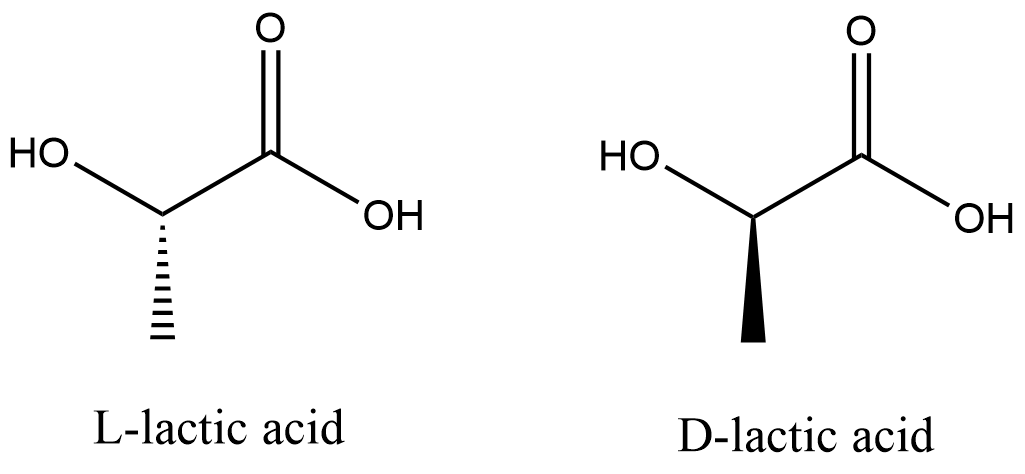
\includegraphics[width=0.5\textwidth]{LA_types.png}
    \caption{L-LA (left) and D-LA (right)}
    \label{fig:LA_types}
\end{figure}

\subsection{Ring opening polymerisation}

Industrial production of \gls{pla} mostly depends on \gls{rop}. This polymerisation reaction starts from lactide which is created starting from \gls{la}. 
There exists three lactides consisting of different stereoisomeric \gls{la} units, namely L-, D- and meso-lactide.  
L- and D-lactides consist of two L- and D-\gls{la}s, respectively, while meso-lactide consists of both L- and D-\gls{la}. Racemic lactide (rac-lactide) is an equimolar mixture of L- and D-lactides\citec{MASUTANI201411}.

\begin{figure}[ht]
    \centering
    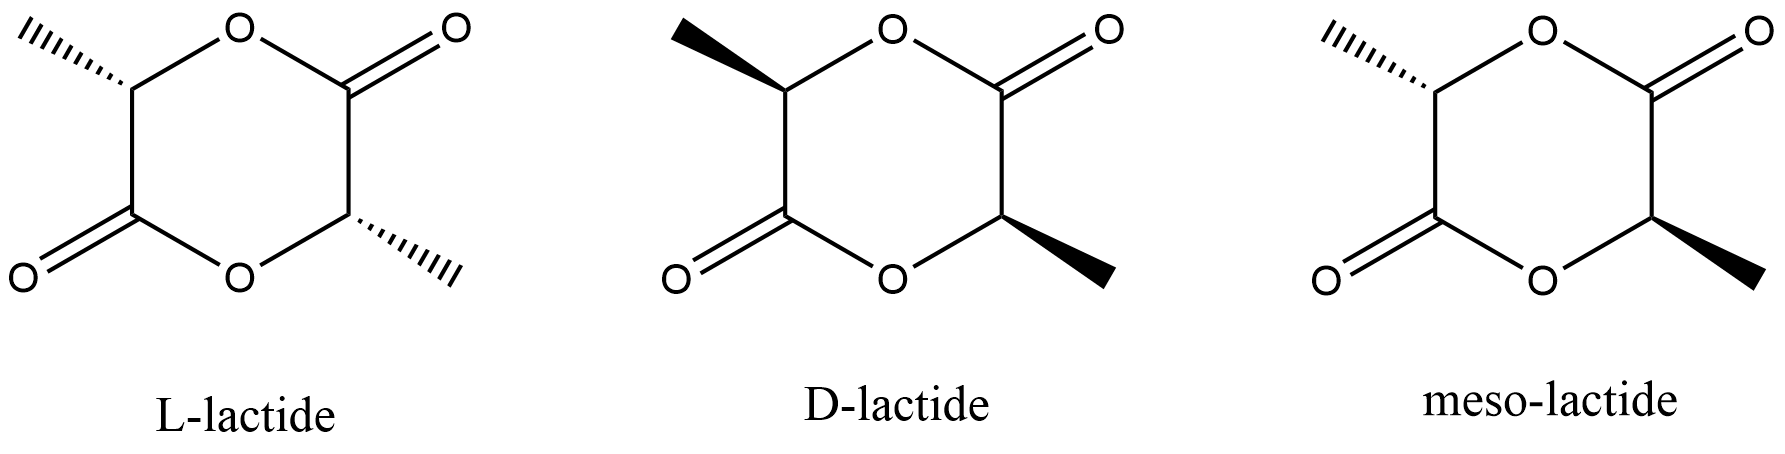
\includegraphics[width=0.8\textwidth]{lactide_types.png}
    \caption{L-lactide (left), D-lactide (middle) and meso-lactide (right)}
    \label{fig:lactide_types}
\end{figure}

The polymerisation of L- and D-lactides gives isotactic homopolymers of \gls{plla} and \gls{pdla}, respectively. Using rac- and meso-lactides for the polymerisation results in optically inactive \gls{pdlla} which has an atactic sequence of L and D units\citec{MASUTANI201411}.

Three reaction mechanisms have been proposed thus far for ROP of lactide: namely anionic, cationic and coordination (also called radical) mechanisms. The anionic and cationic mechanisms have some undesirable side effects and for that reason the coordination mechanism is mostly used. 
Coordination polymerisation with a metal catalyst (mostly alkoxides) can give large molecular weight with a high optical purity. The main principle of how this reaction occurs is seen in figure \ref{fig:PLA_ROP}. (n denotes the amout of lactides added)

\begin{figure}[ht]
    \centering
    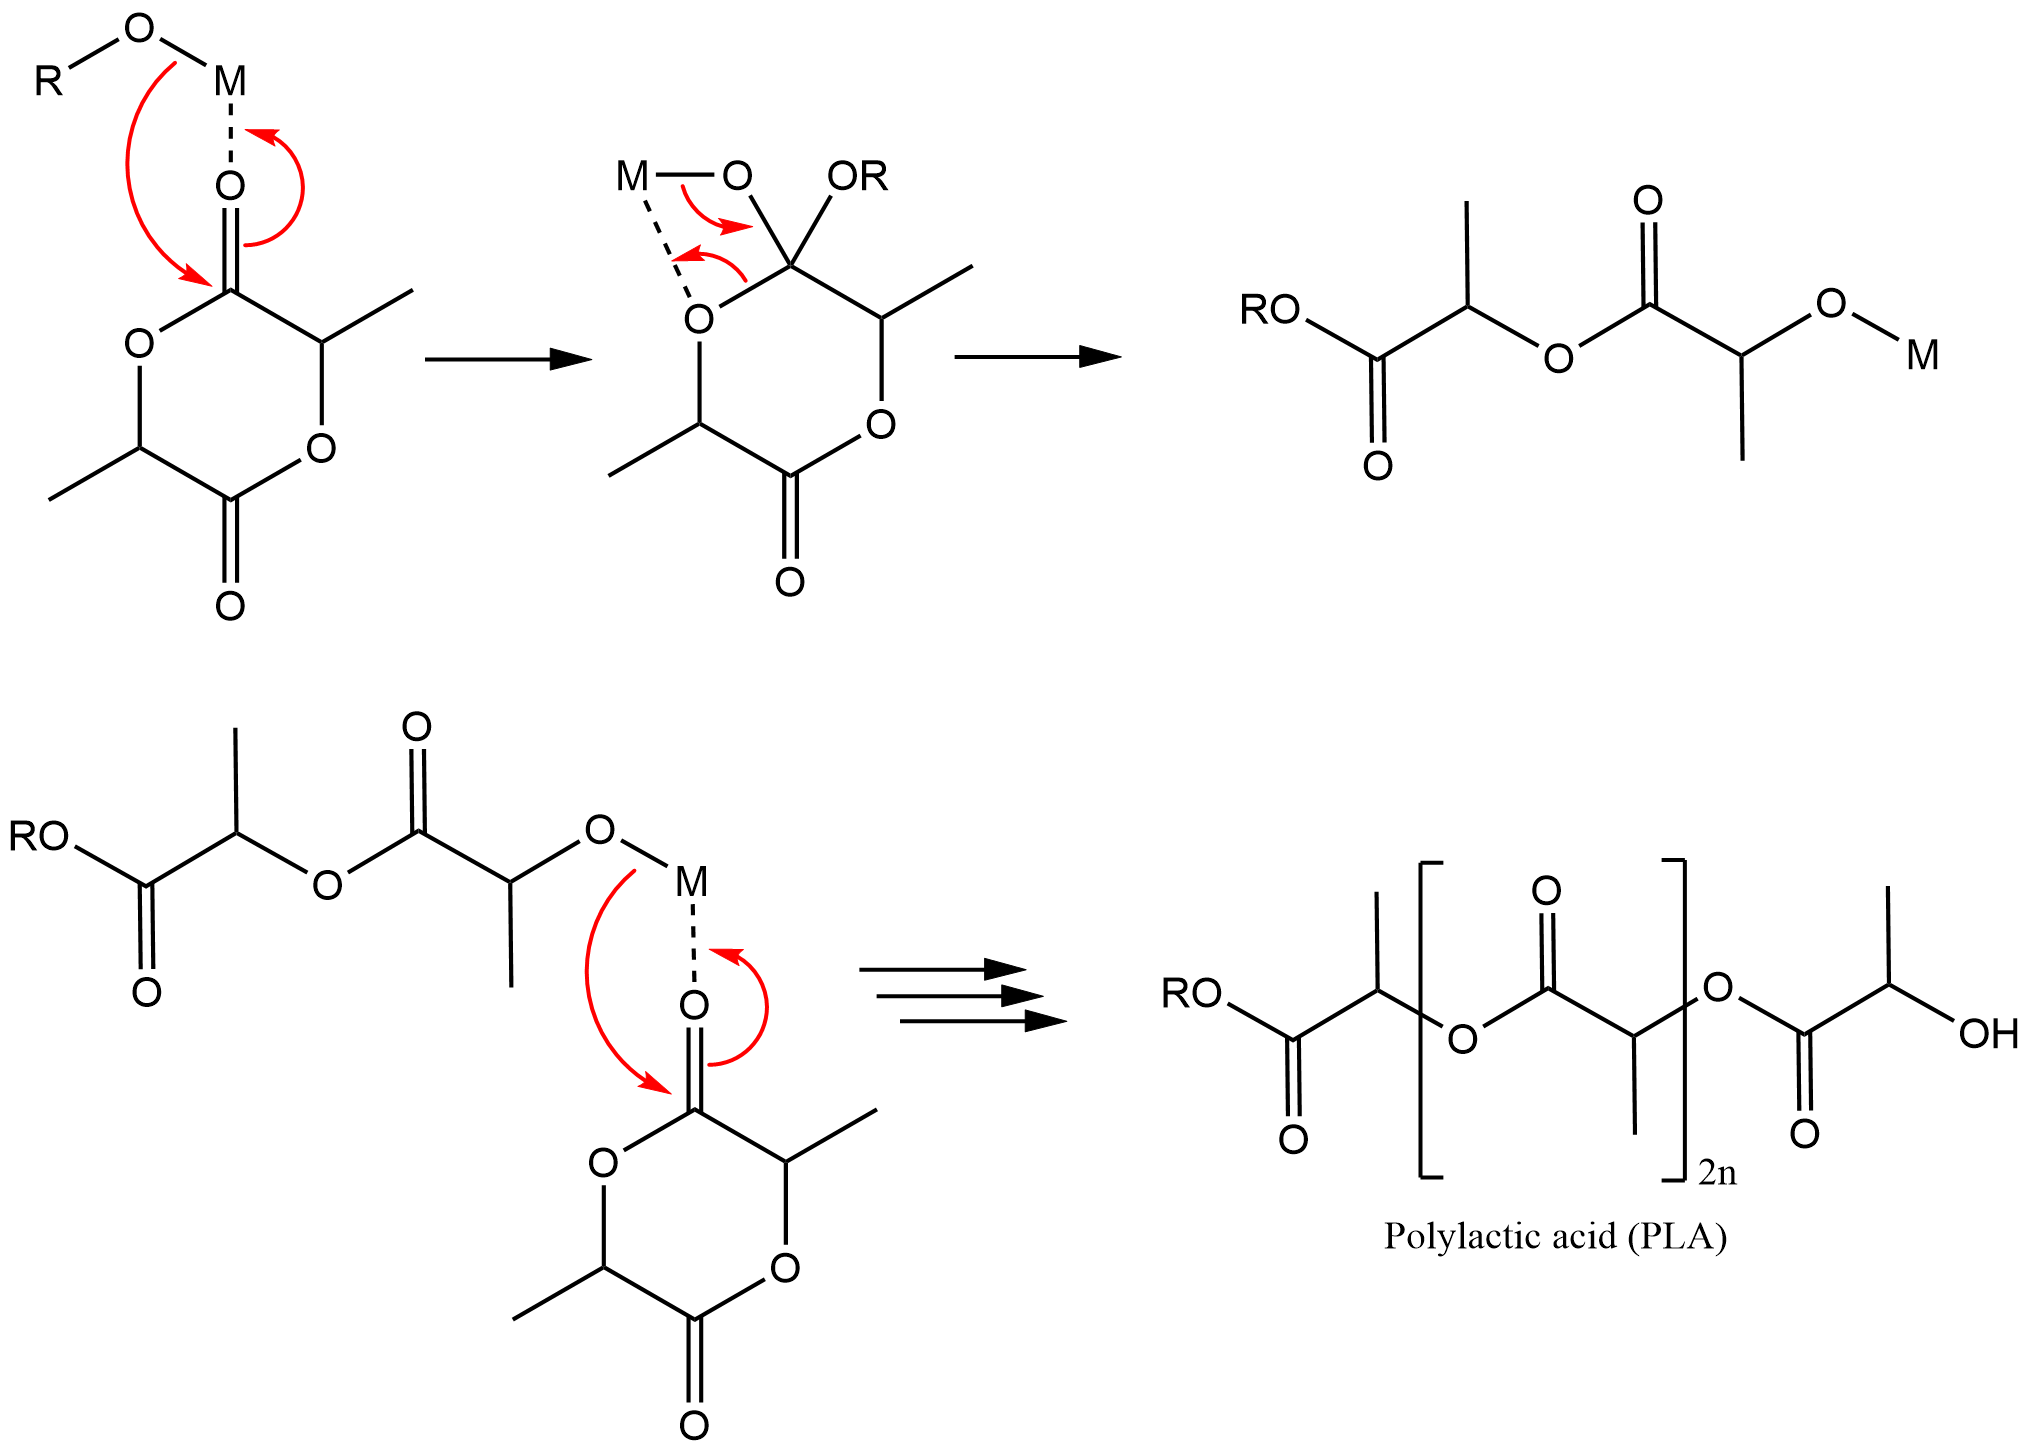
\includegraphics[width=0.8\textwidth]{PLA_ROP.png}
    \caption{ROP of lactide\citec{C0PY00204F}}
    \label{fig:PLA_ROP}
\end{figure}

\subsection{Polycondensation}

The most common mechanism of direct polycondensation of \gls{la} into \gls{pla} is depicted in figure \ref{fig:PLA_condensation}. It is an equilibrium reaction in which \gls{la} molecules bind together, releasing water molecules. Similar as to \gls{rop} does the choice of \gls{la} result in different types of \gls{pla}. 
The pure L- and D-\gls{la} results in \gls{plla} and \gls{pdla}, respectively, while the racemic mixture of the two results in \gls{pdlla}\citec{MASUTANI201411}. 

Polymers produced through direct polycondensation are usually of low molecular weight and low quality. Because of this newly developed polycondensation methods have been proposed such as \gls{ap} and \gls{ssp}. One of the benefits of \gls{rop} over polycondensation is the ability to produce polymers with a wider range of molecular weights by controlling the purity of lactide and the synthesis conditions, without the need for a chain coupling agent or an azeotropic system. 
Therefore, \gls{rop} is still the most common used mechanism in \gls{pla} leading producers\citec{chafran2019}.

\begin{figure}[ht]
    \centering
    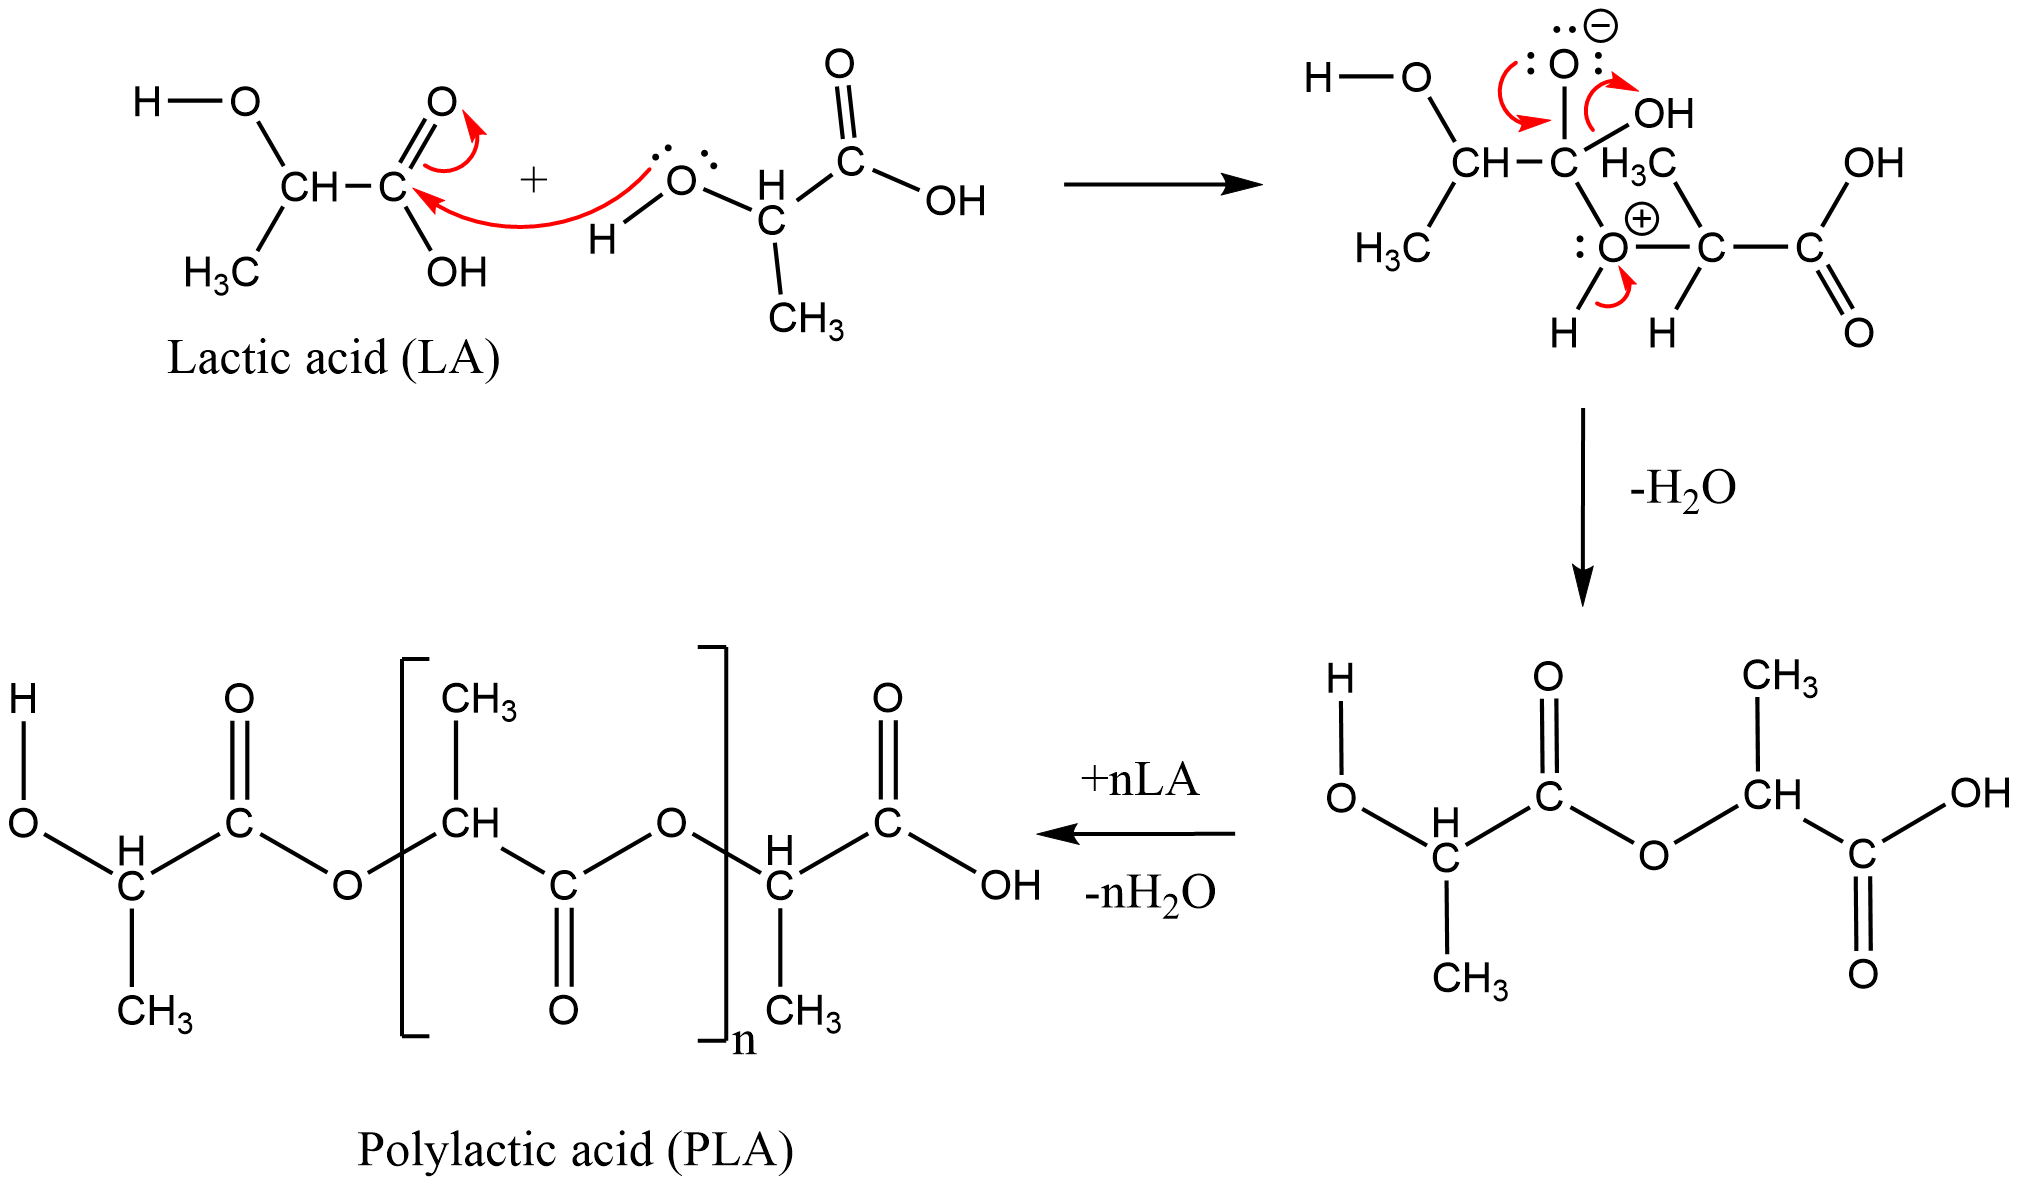
\includegraphics[width=0.8\textwidth]{PLA_condensation.png}
    \caption{Polycondensation polymerisation of PLA}
    \label{fig:PLA_condensation}
\end{figure}
